\mysection[WildStrawberry]{\centering Stetige Funktionen}
\mysubsection{Reellwertige Funktionen}
Sei $D$ eine beliebige Menge. Die Menge $R^D$ aller Funktionen $f:D\rightarrow \mathbb{R}$ bildet einen Vektorraum über $\mathbb{R}$, wobei Addition, skalare Multiplikation, und das Produkt gegeben sind durch: 
\begin{enumerate}
    \item $(f_1+f_2)(x)=f_1(x)+f_2(x)$
    \item $(\alpha \cdot f)(x)=\alpha \cdot f(x)$
    \item $(f_1\cdot f_2)(x)=f_1(x)f_2(x)$
\end{enumerate}
wobei $f_1,f_2,f\in\mathbb{R}^D,x\in D,\alpha\in\mathbb{R}$.

Eine konstante Funktion ist eine, die immer denselben Wert annimt. Darunter gibt es die Funktionen $\mathtt{0},\mathtt{1}\in\mathbb{R}^D$:
\begin{enumerate}
    \item $\mathtt{0}(x)=0\ \forall x\in D$
    \item $\mathtt{1}(x)=1\ \forall x\in D$
\end{enumerate}
Offensichtlich gilt $f+\mathtt{0}=f,g\cdot\mathtt{1}=g\ \forall f,g\in\mathbb{R}^D$. $\mathbb{R}^D$ versehen mit $+,\cdot$ erfüllt die Körperaxiome (ausser: falls $|D|\geq 2$ gibt es immer ein $f\not = \mathtt{0}$, das kein multiplikatives Inverses besitzt.

Auf $\mathbb{R}^D$ definieren wir eine Ordnung: $f\leq g \Leftrightarrow f(x)\leq g(x)\ \forall x\in D$. Weiter gilt $f$ ist nicht negativ $\Leftrightarrow \mathtt{0}\leq f$.

\DEF{Beschränktheit}{Sei $f\in\mathbb{R}^D$. Dann $f(D)=\{f(x)|x\in D\}$ und 
\begin{enumerate}
    \item $f$ ist nach oben beschränkt $\Leftrightarrow f(D)\subseteq\mathbb{R}$ ist nach oben beschränkt.
    \item $f$ ist nach unten beschränkt $\Leftrightarrow f(D)\subseteq\mathbb{R}$ ist nach unten beschränkt.
    \item $f$ ist beschränkt $\Leftrightarrow f(D)\subseteq\mathbb{R}$ ist beschränkt.
\end{enumerate}}

\DEF{Monotonie}{Sei $D\subseteq\mathbb{R}$. Eine Funktion $f:D\rightarrow\mathbb{R}$ ist

(1) monoton wachsend $\Leftrightarrow\ \forall x,y\in D: x\leq y \Rightarrow f(x)\leq f(y)$.

(2) streng monoton wachsend $\Leftrightarrow\ \forall x,y\in D: x<y\Rightarrow f(x)<f(y)$.

(3) monoton fallend $\Leftrightarrow\ \forall x,y\in D: x\leq y\Rightarrow f(x)\geq f(y)$.

(4) streng monoton fallend $\Leftrightarrow\ \forall x,y\in D: x<y\Rightarrow f(x)>f(y)$

(5) monoton $\Leftrightarrow (f$ ist monoton wachsend$) \lor (f$ ist monoton fallend$)$.

(6) streng monoton $\Leftrightarrow (f$ ist streng monoton wachsend$) \lor (f$ ist streng monoton fallend$)$.
}

\NOTE{3.1.3}{Sei $n\in\mathbb{N}$. Sei $f:\mathbb{R}\rightarrow\mathbb{R}$ definiert durch $x\mapsto x^n$. Dann $f$ (streng) monoton wachsend $\Leftrightarrow n\ mod\ 2 = 1$.}

\SA{}{Sei $f:[0,1]\rightarrow[0,\infty)$ monoton. Dann ist das Bild von $f$ immer ein beschränktes Intervall $[a,b]\subset[0,\infty)$ mit $0\leq a\leq b < \infty \Rightarrow f$ nicht surjektiv.}


\mysubsection{Stetigkeit}
\DEF{Stetigkeit in einem Punkt}{Sei $D\subseteq\mathbb{R},x_0\in D$. $f:D\rightarrow\mathbb{R}$ ist in $x_0$ stetig $\Leftrightarrow\ \forall\varepsilon > 0\ \exists\delta > 0:\forall x\in D\ (|x-x_0|<\delta\Rightarrow |f(x)-f(x_0)| < \varepsilon)$.}
\begin{figure}[H]
 \centering
 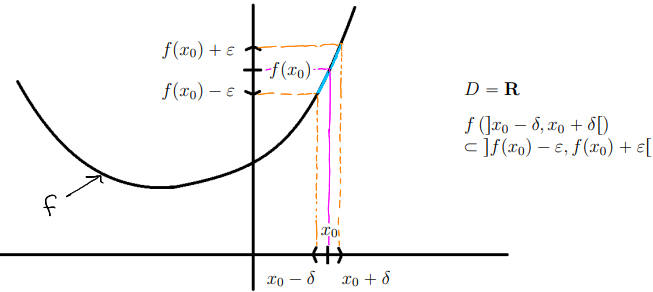
\includegraphics[width=\linewidth,keepaspectratio]{pictures/stetigkeit_in_einem_punkt.png} 
\end{figure}

\DEF{Stetigkeit einer Funktion}{$f:D\rightarrow\mathbb{R}$ ist stetig $\Leftrightarrow f$ ist in jedem Punkt $x\in D$ stetig.}

\SA{3.2.4 Folgenstetigkeit}{Sei $x_0\in D\subseteq\mathbb{R}$ und $f:D\rightarrow\mathbb{R}$ stetig in $x_0$ $\Leftrightarrow\ \forall (a_n)_{n\geq 1}\subseteq D: lim_{n\rightarrow\infty}a_n=x_0\Rightarrow lim_{n\rightarrow\infty}f(a_n)=f(x_0)$.}

\COR{3.2.5}{Sei $x_0\in D\subseteq\mathbb{R},\lambda\in\mathbb{R}$ und $f:D\rightarrow\mathbb{R},g:D\rightarrow\mathbb{R}$ beide stetig in $x_0$.

(1) Dann sind $f+g,\lambda\cdot f,f\cdot g$ stetig in $x_0$.

(2) Falls $g(x_0)\not = 0$ dann ist $\frac{f}{g}:D\cap\{x\in D:g(x)\not =0\}\rightarrow\mathbb{R}$ definiert durch $x\mapsto\frac{f(x)}{g(x)}$ stetig in $x_0$.}

\DEF{Polynomiale Funktion}{Eine polynomiale Funktion $P:\mathbb{R}\rightarrow\mathbb{R}$ ist eine Funktion der Form $P(x)=a_nx^n+...+a_0$ wobei $a_n,...,a_0\in\mathbb{R}$. Falls $a_n\not = 0$ ist $n$ der Grad von $P$.}

\COR{3.2.7}{Polynomiale Funktionen sind auf ganz $\mathbb{R}$ stetig.}

\COR{3.2.8}{Seien $P,Q$ polynomiale Funktionen auf $\mathbb{R}$ mit $Q\not =\mathtt{0}$. Seien $x_1,...,x_m$ die Nullstellen von $Q$. Dann ist $\frac{P}{Q}:\mathbb{R}\ \{x_1,...,x_m\}\rightarrow\mathbb{R}$ definiert duch $x\mapsto\frac{P(x)}{Q(x)}$ stetig.}

\mysubsection{Zwischenwertsatz}
Seien $x_1,x_2\in\mathbb{R}$. Dann liegt $c$ zwischen $x_1$ und $x_2 \Leftrightarrow (x_1\leq x_2 \land c\in[x_1,x_2]) \lor (x_2\leq x_1 \land c\in[x_2,x_1])$.

\SA{3.3.1 Bolzano 1817}{Sei $I\subseteq\mathbb{R}$ ein Intervall, $f:I\rightarrow\mathbb{R}$ eine stetige Funktion und $a,b\in I$. Dann $\forall c$ zwischen $f(a)$ und $f(b)$ gibt es ein $z$ zwischen $a$ und $b$ mit $f(z)=c$.}
\begin{figure}[H]
 \centering
 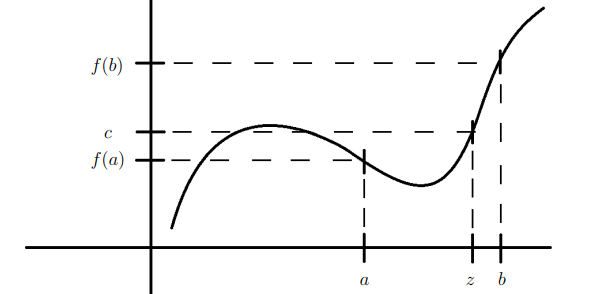
\includegraphics[width=\linewidth,keepaspectratio]{pictures/zwischenwertsatz.png} 
\end{figure}

\COR{3.3.2}{Sei $P(x)=a_nx^n+a_{n-1}x^{n-1}+...+a_0$ ein Polynom mit $a_n\not = 0$ und $n$ ungerade. Dann besitzt $P$ mindestens eine Nullstelle in $\mathbb{R}$.}

\mysubsection{Min-Max Satz}
\DEF{Kompakt}{Ein Intervall $I\subseteq\mathbb{R}$ ist kompakt, falls es von der Form $I=[a,b], a\leq b$ ist.}

\DEF{Notation}{Sei $D$ eine Menge und $f,g:D\rightarrow\mathbb{R}$ Funktionen.
\begin{itemize}
    \item $\forall x\in D: |f|(x):=|f(x)|$
    \item $\forall x\in D: max(f,g)(x):=max(f(x),g(x))$
    \item $\forall x\in D: min(f,g)(x):=min(f(x),g(x))$
\end{itemize}}

\LEM{3.4.3}{Sei $D\subseteq\mathbb{R},x_0\in D$ und $f,g:D\rightarrow\mathbb{R}$ stetig in $x_0$. Dann sind $|f|,max(f,g),min(f,g)$ stetig in $x_0$.}

\LEM{3.4.4}{Sei $(x_n)_{n\geq 1}$ eine konvergente Folge in $\mathbb{R}$ mit $lim_{n\rightarrow\infty}X_n\in\mathbb{R}$. Sei $a\leq b$. Falls $\{x_n:n\geq 1\}\subseteq[a,b] \Rightarrow lim_{n\rightarrow\infty}x_n\in[a,b]$.}

\SA{3.4.5}{Sei $I=[a,b]$. Sei $f:I\rightarrow\mathbb{R}$ stetig. Dann $\exists u,v\in I: f(u)\leq f(x)\leq f(v)\ \forall x\in I \Leftrightarrow f$ ist beschränkt.}

\mysubsection{Satz der Umkehrabbildung}
\SA{3.5.1}{Seien $D_1,D_2\subseteq\mathbb{R}$, $f:D_1\rightarrow D_2,$ $g:D_2\rightarrow\mathbb{R},$ $x_0\in D_1$. Dann $f$ in $x_0$ und $g$ in $f(x_0)$ stetig $\Leftrightarrow g\circ f:D_1\rightarrow\mathbb{R}$ in $x_0$ stetig. }

\COR{3.5.2}{Falls $f$ auf $D_1$ und $g$ auf $D_2$ stetig $\Rightarrow g\circ f$ auf $D_1$ stetig.}

\SA{3.5.3}{Sei $I\subseteq\mathbb{R}$ ein Intervall und $f:I\rightarrow\mathbb{R}$ stetig, streng monoton. Dann ist $J:=f(i)\subseteq\mathbb{R}$ ein Intervall und $f^{-1}:J\rightarrow I$ ist stetig, streng monoton.}

\mysubsection{Reelle Exponentialfunktion}
\SA{3.6.1}{$exp:\mathbb{R}\rightarrow(0,\infty)$ ist stetig, streng monoton wachsend, und surjektiv.}

\DEF{Natürlicher Logarithmus}{Die Umkehrabbildung von $exp:\mathbb{R}\rightarrow(0,\infty)$ ist der natürliche Logarithmus $ln:(0,\infty)\rightarrow\mathbb{R}$.}

\COR{3.6.5}{$ln:(0,\infty)\rightarrow\mathbb{R}$ ist stetig, streng monoton wachsend, und bijektiv.}

\COR{3.6.6}{(1) Für $a>0$ ist $(0,\infty)\rightarrow(0, \infty), x\mapsto x^a$ stetig, streng monoton wachsend, und bijektiv.

(2) Für $a < 0$ ist $(0,\infty)\rightarrow(0, \infty), x\mapsto x^a$ stetig, streng monoton fallend, und bijektiv.}

\mysubsection{Konvergenz von Funktionenfolgen}
Sei $D$ eine Menge. Eine (reellwertige) Funktionenfolge ist eine Abbildung $\mathbb{N}\rightarrow\mathbb{R}^D,n\mapsto f_n$. D.h. jedes $f_n$ ist eine Funktion $D\rightarrow\mathbb{R}$.

Für eine Funktionenfolge schreiben wir $(f_n)_{n\geq 0}$. $\forall x\in D$ erhalten wir eine Folge $(f_n(x))_{n\geq 0}$ in $\mathbb{R}$.

\DEF{Punktweise Konvergenz}{Die Funktionenfolge $(f_n)_{n\geq 0}$ konvergiert punktweise gegen $f:D\rightarrow\mathbb{R}$, falls $\forall x\in D:lim_{n\rightarrow\infty}f_n(x)=f(x)$ $\Leftrightarrow$ $\forall x\in D\ \forall\varepsilon > 0\ \exists N\in\mathbb{N}\ \forall n\geq N: |f_n(x)-f(x)|<\varepsilon$. $f$ ist nicht zwingend in $D$ stetig.}

\DEF{Gleichmässige Konvergenz}{Die Funktionenfolge $f_n:D\rightarrow\mathbb{R}$ konvergiert gleichmässig in $D$ gegen $f:D\rightarrow\mathbb{R}$, falls $\forall\epsilon > 0$ $\exists N\in\mathbb{N}$ s.d. $\forall n\geq N,\forall x\in D: |f_n(x)-f(x)|<\epsilon$ $\Leftrightarrow f_n$ liegt komplett im $\epsilon$-Schlauch um $f$.}

\SA{3.7.4}{Sei $D\subseteq\mathbb{R}$ und $f_n:D\rightarrow\mathbb{R}$ eine Funktionenfolge bestehend aus (in $D$) stetigen Funktionen die (in $D$) gleichmässig gegen $f:D\rightarrow\mathbb{R}$ konvergieren. Falls $f_n$ $\forall n\geq 1$ stetig in $x_0\in D \Rightarrow f$ stetig in $x_0$.}

\COR{3.7.6 Cauchy Kriterium}{Die Funktionenfolge $f_n:D\rightarrow\mathbb{R}$ konvergiert gleichmässig in $D$ $\Leftrightarrow$ $\forall\varepsilon > 0\ \exists N\geq 1$ s.d. $\forall n,m\geq N\ \forall x\in D: |f_n(x)-f_m(x)|<\varepsilon$.}

\COR{3.7.7}{Sei $D\subseteq\mathbb{R}$. Falls $f_n:D\rightarrow\mathbb{R}$ gleichmässig konvergente Folge stetiger Funktionen $\Rightarrow f(x):=lim_{n\rightarrow\infty}f_n(x)$ stetig.}

\mysubsection{Reihen von Funktionen}
\DEF{Konvergenz}{Die Reihe $\sum_{k=0}^{\infty}f_k(x)$ konvergiert punktweise (resp. gleichmässig) in $D$, falls die Funktionenfolge $S_n(x):=\sum_{k=0}^nf_k(x)$ punktweise (resp. gleichmässig) konvergiert.}

\SA{3.7.9}{Sei $D\subseteq\mathbb{R}$ und $f_n:D\rightarrow\mathbb{R}$ eine Funktionenfolge. Sei $|f_n(x)|\leq c_n\in[0,\infty)\ \forall x\in D$ und $\sum_{n=0}^{\infty}c_n$ konvergent. Dann konvergiert $\sum_{n=0}^{\infty}f_n(x)$ gleichmässig in $D$. Falls alle $f_n$ in $D$ stetig sind, dann ist $f(x):=\sum_{n=0}^{\infty}f_n(x)$ eine in $D$ stetige Funktion.}

\SA{3.7.11}{Sei $\sum_{k=0}^{\infty}c_kx^k$ eine Potenzreihe mit $\rho > 0$. Sei $f(x):=\sum_{k=0}^{\infty}c_kx^k,\ |x|<\rho$. Dann gilt $\forall 0\leq r < \rho$ konvergiert $\sum_{k=0}^{\infty}c_kx^k$ gleichmässig auf $[-r,r]$ und $f:(-\rho,\rho)\rightarrow\mathbb{R}$ stetig.}


\mysubsection{Trigonometrische Funktionen}